% This is "sig-alternate.tex" V2.0 May 2012
% This file should be compiled with V2.5 of "sig-alternate.cls" May 2012
%
% This example file demonstrates the use of the 'sig-alternate.cls'
% V2.5 LaTeX2e document class file. It is for those submitting
% articles to ACM Conference Proceedings WHO DO NOT WISH TO
% STRICTLY ADHERE TO THE SIGS (PUBS-BOARD-ENDORSED) STYLE.
% The 'sig-alternate.cls' file will produce a similar-looking,
% albeit, 'tighter' paper resulting in, invariably, fewer pages.
%
% ----------------------------------------------------------------------------------------------------------------
% This .tex file (and associated .cls V2.5) produces:
%       1) The Permission Statement
%       2) The Conference (location) Info information
%       3) The Copyright Line with ACM data
%       4) NO page numbers
%
% as against the acm_proc_article-sp.cls file which
% DOES NOT produce 1) thru' 3) above.
%
% Using 'sig-alternate.cls' you have control, however, from within
% the source .tex file, over both the CopyrightYear
% (defaulted to 200X) and the ACM Copyright Data
% (defaulted to X-XXXXX-XX-X/XX/XX).
% e.g.
% \CopyrightYear{2007} will cause 2007 to appear in the copyright line.
% \crdata{0-12345-67-8/90/12} will cause 0-12345-67-8/90/12 to appear in the copyright line.
%
% ---------------------------------------------------------------------------------------------------------------
% This .tex source is an example which *does* use
% the .bib file (from which the .bbl file % is produced).
% REMEMBER HOWEVER: After having produced the .bbl file,
% and prior to final submission, you *NEED* to 'insert'
% your .bbl file into your source .tex file so as to provide
% ONE 'self-contained' source file.
%
% ================= IF YOU HAVE QUESTIONS =======================
% Questions regarding the SIGS styles, SIGS policies and
% procedures, Conferences etc. should be sent to
% Adrienne Griscti (griscti@acm.org)
%
% Technical questions _only_ to
% Gerald Murray (murray@hq.acm.org)
% ===============================================================
%
% For tracking purposes - this is V2.0 - May 2012

\documentclass{acm_proc_article-me}
\graphicspath{{IMAGES/}}


\input{Notations}
%\newcommand{\mypartitle}[2][2]{\vspace*{-#1 ex}~\\{\noindent {\bf #2}}}

\usepackage{amssymb}
\usepackage{amsfonts}
\usepackage{url}
\usepackage{paralist}
\usepackage{multirow}

\usepackage{amsmath}
\usepackage{algorithm}
\usepackage[noend]{algpseudocode}
\usepackage{listings}

\begin{document}
%
% --- Author Metadata here ---
%\conferenceinfo{\textit{MediaEval 2015 Workshop,}}{Sept. 14-15, 2015, Wurzen, Germany}
%\CopyrightYear{2007} % Allows default copyright year (20XX) to be over-ridden - IF NEED BE.
%\crdata{0-12345-67-8/90/01}  % Allows default copyright data (0-89791-88-6/97/05) to be over-ridden - IF NEED BE.
% --- End of Author Metadata ---

\title{(Provisional) Towards large scale multimedia indexing: \\ A case study on person discovery in broadcast news\\[-100mm]}
%
% We need to keep anonymity for the reviewers
%\author{Nam Le$^{1, 2}$, Alexander Heili$^{1}$, Di Wu$^{1}$, Jean-Marc Odobez$^{1, 2}$\\

\author{}
%% \author{Author 1$^{1, 2}$, Author 2$^{1}$, Author 3$^{1, 2}$\\
%% {\footnotesize %$^1$ \affaddr{Idiap Research Institute, Martigny, Switzerland}}\\
%% $^1$ \affaddr{Affiliation address 1}}\\
%% {\footnotesize %$^2$ \affaddr{\'{E}cole Polytechnique F\'{e}d\'{e}ral de Lausanne, Switzerland}}\\
%% $^2$ \affaddr{Affiliation address 2}}\\
%% %{\footnotesize \email{\{nle, aheili, dwu, odobez\}@idiap.ch}}
%% {\footnotesize \email{\{author1, author2, author3\}@mail.com}}
%% }

\maketitle


\begin{abstract}

Person discovery in the absence of prior identity knowledge requires accurate association of audio-visual cues and detected names. 
%
Clustering-based approach. s
%
With new advances in face andvoice representation, new strategies are proposed, namely verification based, graph-based methods.
%
MediaEval Person Discovery challenge at MediaEval 2016 with the associated corpus.
%
This paper provides quantitative and qualitative comparisons of
these methods. We also investigate why all systems failed for particular shots, paving the way for future promising research directions.

\end{abstract}

\endinput


\section{Introduction}

As the retrieval of information on people in videos is of high interest for users, algorithms indexing identities of people and retrieving their respective quotations are indispensable for searching archives. This practical need leads to research problems on how to index people presence in videos.
%
%TV archives maintained by national institutions such as the French INA, the Netherlands Institute for Sound \& Vision, or the BBC are rapidly growing in size. The need for applications that make these archives searchable has led researchers to devote concerted effort to developing technologies that create indexes.
%
%Because human nature leads people to be very interested in other people.
%Indexes that represent the location and identity of people in the archive are indispensable for searching archives.
%
Started in 2011, the REPERE challenge aimed at supporting research on multimodal person recognition~\cite{BERNARD--SLAM--2013, GIRAUDEL--LREC--2012}. Its main goal was to answer the two questions \emph{``who speaks when?''} and \emph{``who appears when?''} using any available source of information (including pre-existing biometric models and person names extracted from the videos).
%from text overlay and speech transcripts). 
%
Thanks to this challenge and the associated multimodal corpus~\cite{GIRAUDEL--LREC--2012}, significant progresses were achieved in either supervised or unsupervised multimodal person recognition~\cite{BECHET--INTERSPEECH--2014, BREDIN--IJMIR--2014, GAY--CBMI--2014, poignant2012fusion, ROUVIER--CBMI--2014}.

However, when a content is created or broadcast, it is not always possible to predict which people will be the most important to find in the future and biometric models may not yet be available at indexing time.
%
Under real world conditions, this raises the challenge to index people in the archive when there is no pre-set list of people to index.
%
This makes the task completely unsupervised.
%
In order to successfully tag people with the correct identities, names must first be detected from audio-visual sources such as automatic transcripts (ASR) or optical character recognition (OCR).
%
Then one must find a way to assign a name correctly to a presence of the corresponding person, and that name must also be propagated to all the shots during which that person appears and speaks. 
%

A standard approach to solve this is first based on face/speech clustering to partition a videos into homogeneous segments according to identities, followed by the assignment of names to segments appropriately.
%
Although commonly used in state-of-the-art systems~\cite{le2015eumssi,poignant2012fusion}, it suffers from several drawbacks such as potential errors of face/speech clustering or the lack of straightforward way to combine audio-visual streams.
%
In order to alleviate these drawbacks of clustering-based naming %as well as to take advantage of recent advances in verification and 
two alternative strategies are proposed based on verification and graph optimization. 
%
All these three strategies share some common building blocks such as face/speech representation, person diarization, or audio-visual (AV) verification. Though each of these blocks has been well studied within its respective context~\cite{parkhi15deep,wallace2012total,Schroff2015,Ben},
%
they have never been fully investigated and compared as whole systems in  multimedia indexing context before. 

Thus in this paper, we  aim to investigate these approaches with variations in their components using the medium  scale multimedia dataset associated to the ``Multimodal Person Discovery in Broadcast TV'' task~\cite{POIGNANT--MEDIAEVAL--2015,bredin2016mediaeval}.
%
The benchmarking results allow us to analyse all 3 approaches to understand their pros and cons to draw lessons for good practice in large-scale person discovery in broadcast news.

The next Section introduces more details about the Person Discovery challenge, its corpus and evaluation protocol.
Then Section \ref{sec:overview} gives an overview about our approaches while Section \ref{sec:clustering} to \ref{sec:multimodal}
 describe the methodologies in more details.
Section \ref{sec:experiment} presents experiments and analysis, while 
Section \ref{sec:discuss} concludes the paper 
with further discussions.

\endinput


%\input{RelatedWorks}

\section{Person Discovery challenge}
\label{sec:challenge}


The goal of this challenge is to address the indexing of people in archives under real-world conditions when no pre-existing labels or biometric models exist.

\mypartitle{Task overview.} Participants are provided with a collection of TV broadcast recordings pre-segmented into shots.
Each shot $s \in \shots$ has to be automatically tagged with the names of people both speaking and appearing at the same time during the shot: this tagging algorithm is denoted by $\hypLabels : \shots \mapsto \mathcal{P}(\hypNames)$.

The list of persons is not provided \emph{a priori}, and person biometric models (neither voice nor face) cannot be trained on external data. 
The only way to identify a person is by finding their name $n \in \hypNames$ in the audio (\emph{e.g.} using ASR) or visual (\emph{e.g.} using OCR) streams and associating them to the correct person (Fig. \ref{fig:evidence}). %This makes the task completely unsupervised (\emph{i.e.} using algorithms not relying on pre-existing labels or biometric models). 
%Because person names are detected and transcribed automatically, they may contain transcription errors to a certain extent (more on that later in Section~\ref{sec:metric}). 
We denote by $\refNames$ the set of all possible person names in the universe, correctly formatted as \texttt{firstname\_lastname}, while $\hypNames$ is the set of hypothesized names.

\begin{figure}[tb]
 \centering
 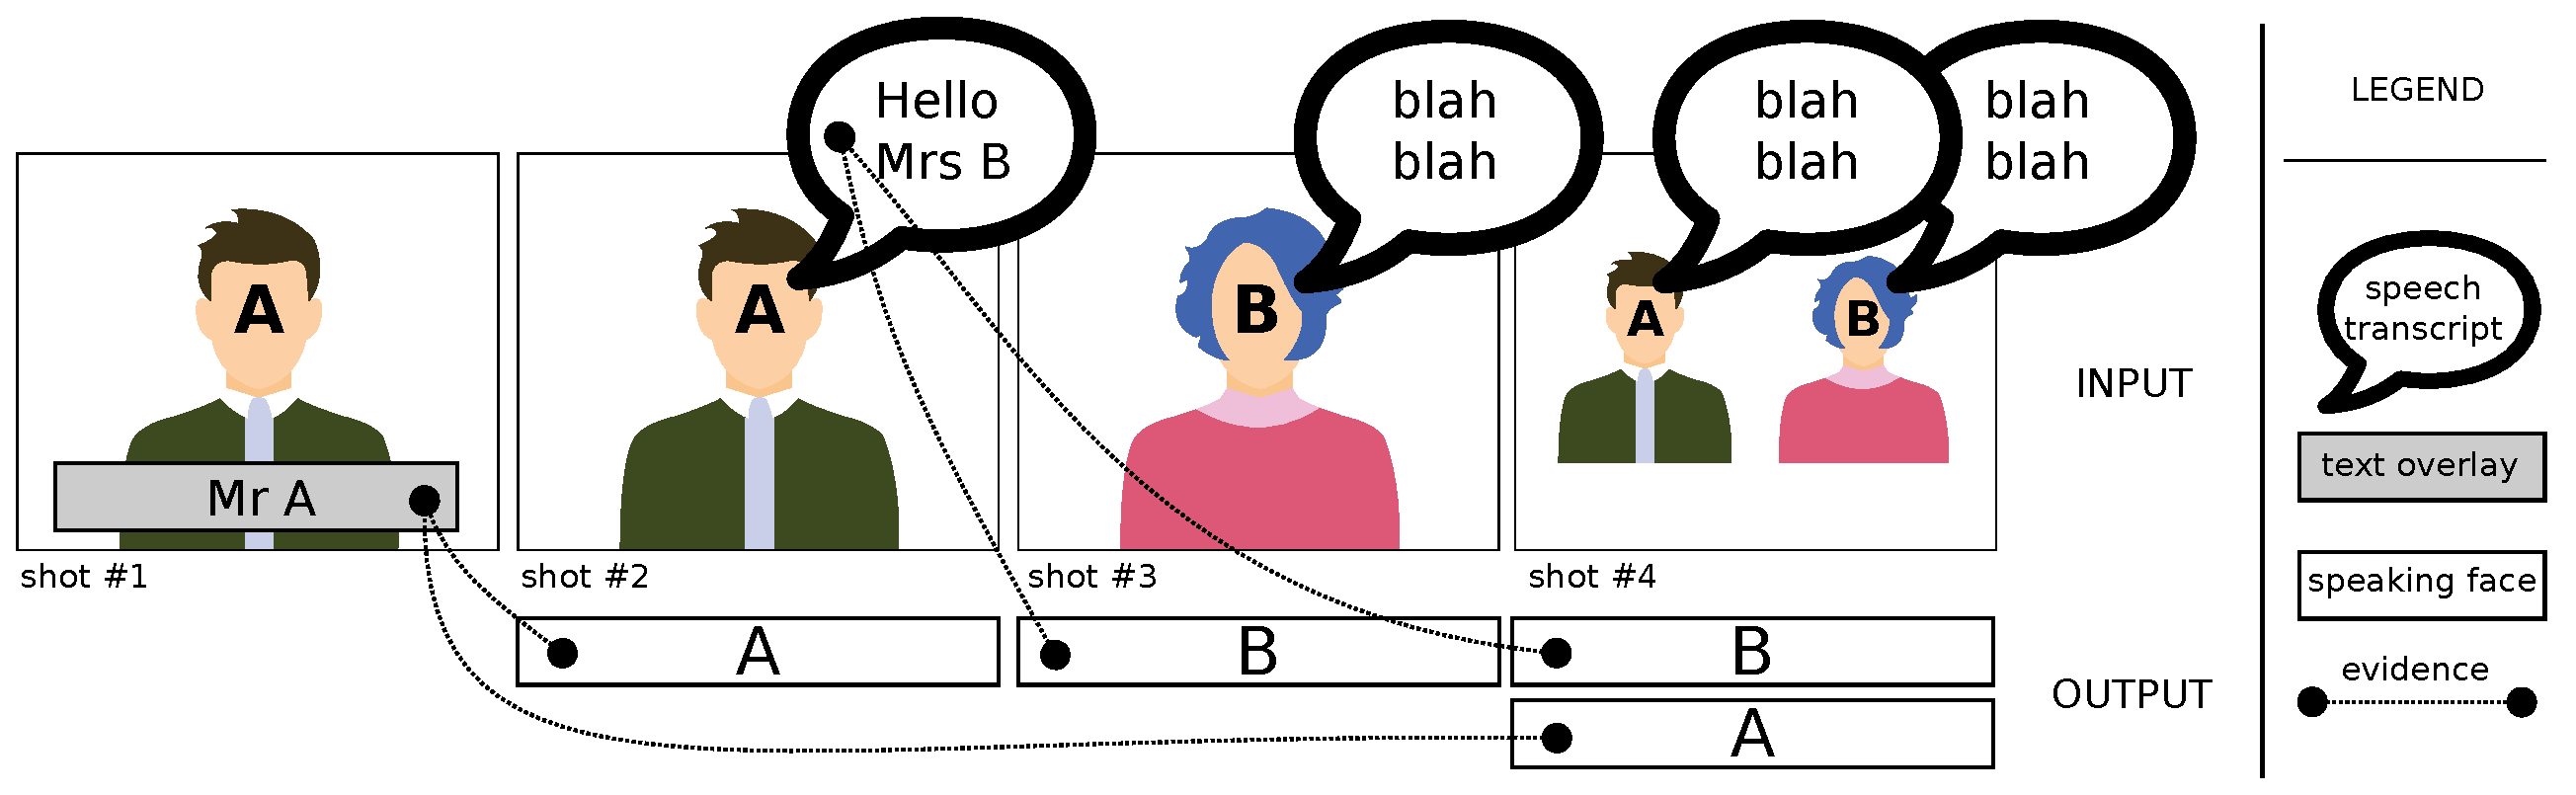
\includegraphics[width=1.\linewidth]{evidence.pdf}
\vspace*{-5mm}
 \caption{For each shot, participants have to return the names of every speaking face. An evidence is also returned for annotation process.}
\vspace*{-3mm}
 \label{fig:evidence}
\end{figure}

\mypartitle{Datasets and annotation.} The test set is divided into three sets: INA, DW, and 3/24. The INA dataset contains a full week of broadcast for two TV french channels (total duration of 90 hours). The DW dataset~\cite{EUMSSI} is composed of video downloaded from the Deutsche Welle website, in English and German for a total duration of 50 hours. The last dataset contains 13 hours of broadcast from the 3/24 Catalan TV news channel. 

Partial annotation was performed to tag each shot with the names of people who appear and speak within that shot using the following approach.
%
From all participant submissions to the challenge, a set of hypotheses were generated for each shot. 
Then participants also engaged in an interactive annotation process.
Detected names were first annotated with  thumbnails which were then used to verify whether people appeared and talked in a particular shot. 
This annotation process yielded 3431 shots with 619 identities annotated (see Tab. \ref{tab:stats} for details).

\begin{table}[tb]
\centering
\caption{Number of identities and corresponding shots where people appear and speak in each set of the corpus.}
\vspace*{-2mm}
\begin{tabular}{c|c|c|c|c|}
\cline{2-5}
    						   		& DW  	& INA 	& 3/24  & Total\\ \hline
 \multicolumn{1}{|c|}{\# shots} 		& 950	& 2250  & 231 & 3431\\ \hline

 \multicolumn{1}{|c|}{\# identities} 	& 344	& 232   & 44 & 619 \\ \hline
								
\end{tabular}
%
\vspace*{-5mm}
\label{tab:stats}
\end{table}



\mypartitle{Metrics.} The task is evaluated indirectly as an information retrieval task. %, using the following principle:
%
For each query $q \in \queries \subset \refNames$, returned shots are first sorted by the edit distance between the hypothesized person name and the query $q$ and then by confidence scores.
The average precision $\text{AP}(q)$ is then computed based on the list of relevant shots (according to the groundtruth) and the sorted list of shots. Finally, the mean average precision (MAP) is computed as follows:
\begin{align}
            \text{MAP} & = \frac{1}{|\queries|} \sum_{q \in \queries} \text{AP}(q) \nonumber
\end{align}

\mypartitle{Video OCR-NER}. As the task we aim at is fully unsupervised, 
the names of people have to be found in the audio or visual streams.
%
%Person identities can be retrieved either from speech transcripts or from overlaid person names commonly used to introduce the current speaker. 
%
Person identification from automatic ASR transcripts usually deteriorates performance. 
Meanwhile, video text can be reliably extracted using OCR and names from overlaid texts often coincide temporally with the people visible and speaking.
%and names of people appearing in the video can be relatively well distinguished in OCR outputs. They can be also associated with people in the video more easily than verifying when whether pronounced names in ASR transcripts refer to people visible in the video. 
Thus, in this work we use only names coming from OCR segments.

For  OCR recognition, we relied on the approaches described in \cite{chen-pr04}.
% for text recognition in videos.
%and on \cite{daddaoua:ICDAR:05} for text recognition and indexing.
%
In brief, first the video is preprocessed with a motion filtering to reduce false alarms, 
and individual frames are processed to localize the text regions.
%
%As compared to printed documents, OCR in TV news videos encounters several challenges: low resolution of text regions, sequence of different texts continuously displayed, or small amount of text to be recognized etc.
%
Then, multiple image segmentations of the same text region are decoded, and all results are compared and 
aggregated over time to produce several hypotheses. 
%Due to the long running time, only the lower half of the videos are processed.
%
The best hypothesis is used to extract people names for identification. Then MITIE open library\footnote{\url{https://github.com/mit-nlp/MITIE}} is used to perform named entity recognition (NER). 
%
%However, detecting names for identification can be more challenging due to several factors: (a) OCR text are often not sentences but short phrases, (b) names come from various languages, and (c) there are names of editorial staff who do not appear within the video, thus are not useful for identification such as cameramen or editors.
%
To improve the raw MITIE results, a rule-based step identifies names not corresponding to introduced people (e.g. editorial staff,  
based on their roles like  cameraman or writer) since they  do not appear within the video.

\section{Overview of our approaches}
\label{sec:overview}

Conventional approaches for person recognition rely on face and/or voice biometric models.
Thus, a very large amount of trained models is needed to cover only a decent percentage of all the people in
TV shows.
%
In addition, it is not always possible to predict which people will be the most important to find in the future.
%
To solve these problems, detected people names are assigned to faces and voices following the basic principle 
that occurrences of similar faces and voices should have the same name.
%
Below, we briefly introduce the 3 different paradigms used in of this paper  to solve the task,
which have different characteristics (generative vs. discriminative models, pairwise verification vs. global optimization, etc.), 
while later sections provides more details about them.
%

\mypartitle{Clustering-based naming (CBN).} This is the most common approach. Face/speech tracks are first aggregated into homogeneous clusters according to person identities. Then each cluster is tagged with the most probable person name (Fig.\ref{fig:cbn}). 
This approach heavily depends on the  clustering quality and granularity: 
a large number of clusters can significantly reduce the 
indexing recall, while a too small number may produce false alarms and affect the indexing precision (\textit{i.e.} over-clustering).


\mypartitle{Verification-based naming (VBN).} To overcome the weakness of CBN, 
VBN puts higher priority on detected names, and proceed in two main steps (Fig.~\ref{fig:vbn}).
%
A person enrolment step relying on face/speech tracks reliably associated with OCR names, 
and a verification step on all other face/speech segments, which implictly ranks them according to the identity.


\mypartitle{Graph-based naming (GBN).} 
VBN propagates names based on a one-one distance while in CBN, all the distances are globally considered. 
Graph-based naming is thus proposed as an hybrid approach between them.
%
A graph is built using  face/speech tracks as a nodes and AV similarities between nodes as edge weights. 
As in VBN, some nodes are initially tagged with the names, and this information is then propagated along the edges 
within the graph (Fig.~\ref{fig:gbn}).


\endinput


\section{Video OCR and NER}
\label{sec:ocr_ner}
As the task we aim at is full unsupervised, i.e. list of people is not provided in advance, their names have to be found in the audio (\emph{e.g.}, using speech transcription -- ASR) or visual (\emph{e.g.}, using optical character recognition -- OCR) streams.
%
%Person identities can be retrieved either from speech transcripts or from overlaid person names commonly used to introduce the current speaker. 
%
Person identities from transcripts deteriorates when transcripts come from automatic speech recognition. Meanwhile, text can be reliably extracted using OCR techniques, and their association with people in the videos is easier than analysing whether or not pronounced names in ASR transcripts actually refer to people appearing in the video. Thus, in this work we use only names coming from OCR segments in videos.

To detect OCR segments in videos and exploit them for retrieval, we first relied on the approaches described in \cite{chen-pr04,odobez-prl05} for text recognition in videos, and on \cite{daddaoua:ICDAR:05,vincia:tmm:05} for text recognition and indexing.
%
In brief, given an input video, two main steps are applied: first the video is preprocessed with a motion filtering to reduce noise, and individual frames are processed to localize and binarize the text regions for text recognition.
%
As compared to printed documents, OCR in TV news videos encounters several challenges: low resolution of text regions, sequence of different texts continuously displayed, or small amount of text to be recognized etc.
%
To tackle these, multiple image segmentations of the same text region are decoded, and then all results are compared and aggregated over time to produce several hypotheses. 
%Due to the long running time, only the lower half of the videos are processed.
%
The best hypothesis is used to extract people names for identification. To recognize names from texts, we use the MITIE open library~\footnote{\url{https://github.com/mit-nlp/MITIE}}, which provides state-of-the-art NER tool. 
%
%However, detecting names for identification can be more challenging due to several factors: (a) OCR text are often not sentences but short phrases, (b) names come from various languages, and (c) there are names of editorial staff who do not appear within the video, thus are not useful for identification such as cameramen or editors.
%
To improve the raw MITIE results, a heuristics preprocessing step identifies names of editorial staff based on their roles (cameraman, editor, or writer) because they do not appear within the video, thus are not useful for identification.

\endinput


\section{Clustering-based naming}
\label{sec:clustering}

In this approach, a video must be segmented into homogeneous clusters according to person identity using face clustering and speaker diarization. Then, the clusters are combined with the detected names to compute the optimal assignment (Fig.~\ref{fig:cbn}).

\begin{figure}[!htb]
 \centering
 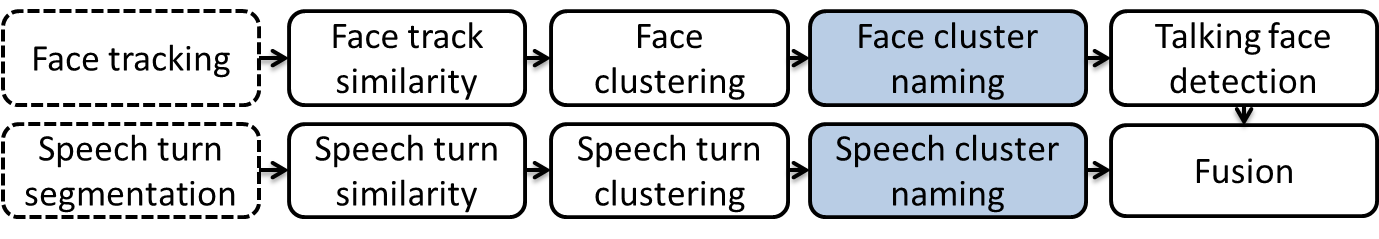
\includegraphics[width=1.\linewidth]{CBN.png}
\vspace*{-5mm}
 \caption{Clustering-based naming process. Light blue boxes are when names are combined with clusters.}
\vspace*{-5mm}
 \label{fig:cbn}
\end{figure}

\subsection{Face clustering}

Given the video shots, face clustering process consists of (i) face detection, detecting faces appearing within each shot, (ii) face tracking, extending detections into continuous tracks within each shot, and (iii) face clustering, grouping all tracks with the same identity into clusters.

\subsubsection{LIMSI system}

Face tracking-by-detection is applied within each shot using a detector based on histogram of oriented gradients~\cite{Dalal2005} and the correlation tracker proposed by \emph{Danelljan et al.}~\cite{Danelljan2014}. 
%
Each face track is then described by its average \emph{FaceNet} embedding and compared with all the others using Euclidean distance~\cite{Schroff2015}. 
%
Finally, average-link hierarchical agglomerative clustering is applied. Source code for this module is available in \emph{pyannote-video}\footnote{\url{http://pyannote.github.io}}.

\subsubsection{EUMSSI system}

A fast version of deformable part-based model (DPM)~\cite{dubout2013deformable} is first applied. Then tracking is performed using the CRF-based multi-target tracking framework~\cite{heili2014tracking}, which relies on the unsupervised learning of time sensitive association costs for different features.
%
The detector is only applied 4 times per second and an explicit false alarm classifier at the track level is learned\cite{Le_ICPR_2016}.
%
Each face track is then described using a combination of keypoint matching distances and total variability modeling (TVM)~\cite{wallace2012total,Khoury:ICMR:2013}.

\subsection{Speaker diarization}

The speaker diarization system (``who speak when?") is based on the LIUM Speaker Diarization system\cite{rouvier2013}, freely distributed\footnote{\url{www-lium.univ-lemans.fr/en/content/liumspkdiarization}}. 
%This system has achieved the best or second best results in the speaker diarization task on REPERE French broadcast evaluation campaigns 2012 and 2013~\cite{galibert2013b}.
%
The diarization system is first composed of an acoustic Bayesian Information Criterion (BIC)-based segmentation followed by a BIC-based hierarchical clustering. Each cluster represents a speaker and is modeled with a full covariance Gaussian. A Viterbi decoding re-segments the signal using GMMs with 8 diagonal components learned by EM-ML, for each cluster. 
%Segmentation, clustering and decoding are performed with 12 MFCC+E, computed with a 10ms frame rate. 
Music and jingle regions are removed using a Viterbi decoding with 8 GMMs (trained on french broadcast news data) for music, jingle, silence, and speech. %(with wide/narrow band variants for the last two, and clean or noised or musical background variants for wideband speech).
%
%In the above steps, features were used unnormalized in order to preserve information on the background environment, which may help differentiating between speakers. 
At this point each cluster contains the voice of only one speaker, but several clusters can be related to a same speaker. The background environment contribution must be removed from each GMM cluster, through feature gaussianization.
%
Finally, the system is completed with clustering method based on the i-vectors paradigm and Integer Linear Programming (ILP). 
This clustering method is fully described in~\cite{rouvier12-2}. 
%The ILP clustering along with i-vectors speaker models gives better results than the usual hierarchical agglomerative clustering based on GMMs and cross-likelihood distances~\cite{Barras2006}.

\subsection{Name assignment}

After obtaining homogeneous clusters during which distinct identities speak or appear, one needs to assign each name output from NER module to the correct clusters. 
%
%However, associating auditory voices with visual person clusters or names has two major difficulties. 
%The visible person may not be the current speaker and the speaking person can be dubbed by a narrator in a different language.
%
%Because of these problems of AV association, 
We use a direct naming method~\cite{poignant2012fusion} which finds the mapping between clusters and names to maximize the co-occurrences between them.
%
Names are propagated based on the outputs of face diarization and speaker diarization independently. 
%
%The direct naming method is applied to speaker clusters to produce a mapping between names and clusters. All shots which overlap with the clusters are tagged with the corresponding names with equal confident scores. 
%
%The same direct method is applied to face clusters to produce a set of named clusters.
%Unlike speaker naming, for  one shot, 
A name coming from face naming is ranked based on the talking score of the cluster's segment within that shot.
%
The talking score is predicted using lip motion and temporal modeling with LSTM~\cite{Le_ACMMM_2016}.

\endinput


\section{Verification-based naming}
\label{sec:verification}


The proposed system can be divided in an enrolment and a search stage. For each person name detected by optical character recognition (OCR), the most likely interval
of speech and face presence are detected and used for enrolment.
%, as depicted in Figure \ref{fig:timeline}. 
Once the detected people are enrolled, speaker and face recognition
are performed for each shot in order to assign labels to that shot. 
A decision fusion strategy is implemented in order to combine the speech and video labels (Fig.~\ref{fig:vbn}). The details of the system
are described below.

\begin{figure}[!htb]
 \centering
 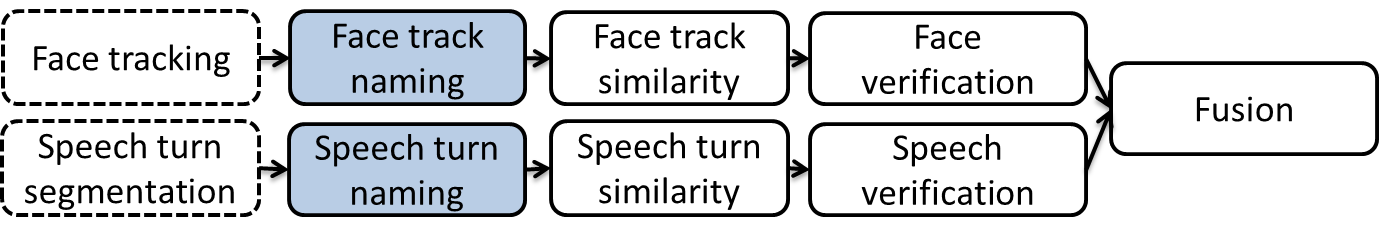
\includegraphics[width=1.\linewidth]{VBN.png}
\vspace*{-5mm}
 \caption{Verification-based naming process. Light blue boxes are when names are combined with face tracks and speech turns to create enrollment models.}
\vspace*{-5mm}
 \label{fig:vbn}
\end{figure}

\subsection{Enrollment}

\subsubsection{GTM-UVigo system}
First, audio and video features were extracted from the recordings. The audio features were 19 MFCCs plus delta, acceleration and energy. For the video features, first
the LIMSI approach was used to detect faces, and then discrete cosine transform (DCT) features were extracted and normalized with Bob toolkit \cite{bob2012}.
%using blocks of size 12
%with 50\% overlap and 45 DCT comonents using the Bob toolkit \cite{bob2012}, preceeded by %geometric normalization and photometric enhancement using the Tan\&Triggs algorithm
%\cite{tan2010}.

For each person name detected by the OCR, the intervals of voice activity detection and appearance of that person were extracted. For the audio, 
the time interval $(t_{\mathrm{start}},t_{\mathrm{end}})$ in which the name of the speaker $spk$ appears is taken as a starting point. A strategy to enlarge this time
 interval in order to obtain more data to enroll the speaker is applied: the boundaries $(t_{\mathrm{start}},t_{\mathrm{end}})$ are iteratively extended $10ms$ to each direction until a change point is detected using the BIC algorithm
for speaker segmentation.
%
% given the time intervals $S_{\mathrm{left}} = (t_{\mathrm{start}}-10,t_{\mathrm{end}})$ and 
% $S_{\mathrm{right}} = (t_{\mathrm{start}},t_{\mathrm{end}}+10)$, a change point is searched within each of these intervals using the Bayesian information criterion algorithm
% (BIC) for speaker segmentation,  having the restriction that the change point has to be in the 
% intervals $(t_{\mathrm{start}}-10,t_{\mathrm{start}})$ and $(t_{\mathrm{end}},t_{\mathrm{end}}+10)$, respectively. If no change point was found within the interval
% $S_{\mathrm{left}}$ then $t_{\mathrm{left}}$ is set to $t_{\mathrm{start}}-10$ and, similarly, if no change point was found within the interval 
% $S_{\mathrm{right}}$ then $t_{\mathrm{right}}$ is set to $t_{\mathrm{end}}+10$. Then, speaker $spk$ is assumed to be speaking in the interval 
% $S_{\mathrm{spk}} = (t_{\mathrm{left}},t_{\mathrm{right}})$. 
% 

For the video, the faces detected by the face tracker in the interval $(t_{\mathrm{start}},t_{\mathrm{end}})$ in 
 which the name of the speaker $spk$ appears were considered.
 %; given that only one face was detected, the whole presence interval of that face is taken but, 
 In case more than one face was detected, the one that appeared in more frames was assigned to the speaker.
 %, assuming that was the dominant face in the given time interval.
 %In case the person appears several times in the OCR output, a segment is computed for each occurrence.
 %
 
 Once the intervals of appearance are defined, an i-vector \cite{dehak10} is extracted for each modality using Kaldi toolkit \cite{kaldi}; in the case of speech, speech activity detection (SAD) was performed beforehand, in order to remove the non-speech intervals. In case several segments were available for a person name, their features were concatenated into a single one.
 %and all the segments  were treated as a single one.

\subsubsection{UPC system}

Using the OCR-NER output, we extracted the \textit{speaker segments/face tracks} temporally overlapping with a written name. These tracks are named 
%with the identity given by the written name 
and will be used to create models for the named person in an unsupervised enrolment step. The models, consisting in a feature vector and a name label, are used to train a verification system.

Speaker information was extracted using an i-vector based speaker tracking system. 
%Assuming that text names are temporarily overlapped with their speaker and face identities, speaker models were created using the data of those text tracks. 
%The baseline speaker diarization was used to select speaker turn segments assigned to OCR names so as to extract the i-vector queries. 
Speaker modelling was implemented using i-vectors \cite{dehak10}. For the feature extraction, 20 MFCCs plus delta and acceleration coefficients were extracted. Using the Alize toolkit\cite{Bonastre1}, a total variability matrix has been trained per show. Therefore, a 400 size i-vector has been extracted for the speaker turn of each query. Those queries with a speaker turn duration beyond 3 seconds were discarded.

We extracted the features from the activation of the last fully connected layer of VGG-face~\cite{parkhi15deep} Convolutional Neural Network (CNN) to train a triplet network architecture~\cite{Schroff2015} using the XXXX face database. An autoencoder was used to reduce the dimensionality of the VGG vectors to 1024. The features from each of the detected faces in each track were extracted and then averaged to obtain a single feature vector.

\subsection{Search}

\subsubsection{GTM-UVigo system}

In order to decide which speaker was present in a shot, first speech and face detection were performed. Speech detection was carried out using a logistic regression approach
used to classify a segment as speech or non-speech, discarding the non-speech segments. For the video, the faces detected by the face tracker within the shot were identified, 
and the one that appeared in more frames (if any) was chosen. After that, the same procedure as in the enrolment stage was performed: features were extracted from the shot
and an i-vector was extracted for each modality (in the case of speech, this was preceded by speech activity detection). Once the i-vectors of the shot were obtained,
cosine scoring with the enrolment i-vectors was computed, choosing the person names that achieved the highest score for each modality. The shot was assigned to
a person if 
%the name assigned by the face and speech modalities were equal and the sum of 
the scores were greater than a threshold.

\subsubsection{UPC system}

For the speech modality, target i-vectors have been extracted from $3s$ segments with a $0.5s$ shift. The identification was performed evaluating the cosine distance of the i-vectors with each query i-vector. The query with the lowest distance was assigned to the segment. A global distance threshold was previously trained with the development database to discard assignations with high distances.

For the video modality, using the set of named tracks from the full video corpus, a Gaussian Naive Bayes (GNB) binary classifier model was trained, using the euclidean distance between pairs of samples from the named tracks. Then, for each specific video, each unnamed track was compared with all the named tracks of the video, computing the euclidean distance between the respective feature vectors of the tracks. This value was classified using the GNB to either being a intra-class distance (both tracks belong to the same identity) or an inter-class distance (the tracks are not from the same person). The probability of the distance being intra-class was used as the confidence score. The unnamed track was assigned the identity of the most similar named track. A threshold on the confidence score (0.75) was used to discard tracks not corresponding to any named track.

\endinput


\section{Graph-based naming}
\label{sec:graph}

%The MOTIF team (IRISA/Inria-Rennes and PUC Minas) considered a graph-based approach for naming the people which are both visible and heard (``speaking faces''). 
In this approach, all the \textit{speaking faces} of a video are the nodes of a complete and undirected graph $\mathcal{G}$, and each edge between two nodes is weighted by the similarity between their respective voices and/or the face tracks.
% The weight matrix $\mathbf{W}$ is therefore symmetrical. 
An initial tagging is done by associating to each face track the co-occurring name(s). Then propagation is performed according to the weights of the graphs using two different strategies, namely MOTIF-RW and MOTIF-MST (Fig.~\ref{fig:gbn}).

\begin{figure}[!htb]
 \centering
 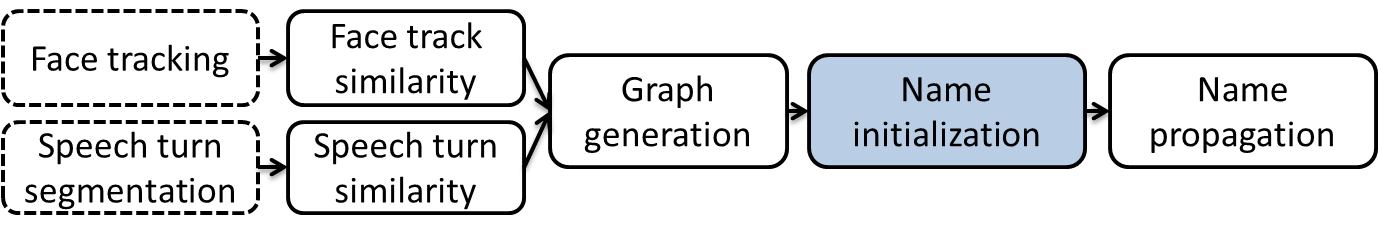
\includegraphics[width=1.\linewidth]{GBN.png}
\vspace*{-5mm}
 \caption{Graph-based naming process. Light blue boxes are when nodes in graph are initiated with names.}
\vspace*{-5mm}
 \label{fig:gbn}
\end{figure}

\subsection{Graph generation details}
\label{ssec:graph_gen}
A node is created for every \textit{speaking face} detected, namely when a face track temporally overlaps a speech segment by at least 60\%. If several speech segments overlap it, the face track is associated the one with the most overlapping one.
%
Edges between nodes are weighted using a measure of similarity deriving from the voice and/or face track similarities.

We compute the visual similarity $\sigma^V_{ij}$ as the cosine between the FaceNet embedding vectors $v_i$ and $v_j$ related to the face tracks of two nodes $N_i$ and $N_j$: $\sigma^V_{ij}=1/2+\frac{v_i\cdot v_j}{||v_i||*||v_j||}$, where $\cdot$ is the dot product and $||.||$ is the L2 norm.

The similarity $\sigma^A_{ij}$ between the speech segments of two nodes  $N_i$ and $N_j$ is computed as follows. Each speech segment is modelled with a 16-GMMs over MFCC features. An Euclidean-based approximation of the KL2 divergence, noted $\delta^A_{ij}$, is then computed between the two GMMs~\cite{Ben}, and turned into a similarity according to $\sigma^A_{ij}=\exp(\log{(\alpha)} \; \delta^A_{ij})$, where $\alpha = 0.25$.
%
The way two modalities can be combined is described in Sec. \ref{sec:multimodal}
%Section 6.2 describes how these similarities are combined into one, $\sigma^{AV}$, to fuse the .

\subsection{Name propagation}

Two different approaches are considered for the propagation of the initial tags: a random walk approach and a hierarchical one based on Kruskal's algorithm. In both cases, every node is associated a particular tag with a confidence score at the end of the propagation phase.

\subsubsection{Random walk (RW)}

This method implements a random walk algorithm with absorbing states, adapting~\cite{zhu2002}. Let $n$ be the number of nodes of $\mathcal{G}$, we compute the probability transition matrix $\mathbf{P}^0$ between all the nodes as $\mathbf{P}^0 = \mathbf{D}^{-1}\mathbf{W}$ where $\mathbf{D}$ is the diagonal {\it degree matrix} where $\mathbf{D}_{ii} = \sum_j \mathbf{W}_{ij}$, $1\leq i \leq n$. Nodes which are already tagged in $\mathbf{P}^0$ are set as \textit{absorbing states}, \textit{i.e.} if $i$ is a tagged node, $\mathbf{P}^0_{ii} = 1$ and $\mathbf{P}^0_{ij} = 0$. The random walk iteration is performed according to $\mathbf{P}^{t+1} = (1-\gamma) ~\mathbf{P}^0 ~ \mathbf{P}^{t} + \gamma ~\mathbf{P}^0$, where $\gamma$ is a parameter enforcing consistency with the initial state and slows down the walk (here $\gamma = 0.5$). When the random walk has converged, let $T$ be the final number of iterations. Each untagged node $u$ is then associated a tagged one $l^*$, where $l^*=\argmax_l{\mathbf{P}^{T}_{ul}}$. $\mathbf{P}^{T}_{ul^*}$ is considered as the confidence score related to the tagging of node $u$.

\subsubsection{Minimum spanning tree (MST)}
This method is based on the computation of a minimum spanning tree, using Kruskal's algorithm. The MST establishes a hierarchical partition of a set \cite{perret2015}. A new connected graph $\mathcal{G'}$ is derived from $\mathcal{G}$ with the same nodes but edge weights representing distances between them (functions of their respective similarities $\sigma^{AV}$). To propagate the initial tags, we start from a null graph $\mathcal{H}$ consisting in the nodes of $\mathcal{G'}$ only, and the following process is repeated, until all edges of $\mathcal{G'}$ are examined: from $\mathcal{G'},$ the unexamined edge $e$ corresponding to the smallest distance is chosen. If it does not link different trees in \color{black}$\mathcal{H}$\color{black},  skip it; otherwise, it links trees $T_1$ and $T_2$ (thus forming  $T_3$), and $e$ is added to the minimum spanning forest $\mathcal{H}$ being created. Three cases are possible: 
\textbf{I.}  None of $T_1, T_2$ is tagged: $T_3$ will not be tagged \textbf{II. } Only $T_1$ is tagged, with confidence score $C_{T_1}$: $T_1$'s tag is assigned to the entire  $T_3$ (\textit{i.e.,} to all its unlabelled nodes), with a confidence score $C_{T_3} = C_{T_1}\times(1-w_e), $ where $w_e$ is the weight of $e$ \color{black} in $\mathcal{G'}$. \color{black} \textbf{III. } Both $T_1$ and $T_2$ are tagged: one of the tags (of $T_1$ or of $T_2$) is picked (at random), and assigned to  $T_3$ with confidence scores as in case II. 


\endinput

\section{Multimodal improvements}
\label{sec:naming}

As names are propagated based on the outputs of face and speech processing modules independently in CBN and VBN, we employed a fusion strategy to aggregate the results. Meanwhile, it is more straightforward to combine 2 modalities in GBN.

\mypartitle{Late fusion ranking.} Let $S = \{s_k\}$ be the list of testing shots. Within each shot, $\{N^F_i, t(N^F_i)\}$ is the set of names returned by face naming and the corresponding talking scores and $\{N^A_i, 1.0\}$  is the set of names returned by speaker naming, each is ranked equally with score 1.0.
%
The names which the two methods agree on are ranked highest. 
%
Then, names from face naming are ranked higher than speaker naming  because we found that face naming is more reliable in empirical experiments.
%
%Alternative strategies that rank speaker naming equal or higher than face naming gave inferior results.
%
The same late fusion strategy is applied to both clustering-based naming and verification-based naming.

\mypartitle{Audiovisual similarity.} For the graph-based approach, the audio and visual modalities can be combined straightforwardly into one similarity.
%
Thus the distance is extended to multi-modality by using a linear combination of the audio and visual similarities defined in section \ref{ssec:graph_gen}: $\sigma^{AV}_{ij} = \beta \sigma^V_{ij} + (1-\beta) \sigma^A_{ij}$. $\beta$ is set experimentally to 0.5.

\endinput

\begin{algorithm}
  \caption{Ranking names within shots
    \label{algo:ranking}}
  \begin{algorithmic}[1]
	  \For{$s_k \in S$}
 	  	    \State{$Q_{s_k} = \emptyset$}
		    \State{Face\_naming$(s_k) \Rightarrow (N^F_i, t(N^F_i))$}
				\State{Speaker\_naming$(s_k) \Rightarrow (N^A_j, 1.0)$}
				\For{each $N^F_i$}
					\If{$\exists N^A_j / N^A_j = N^F_i$}
						\State{$Q_{s_k} = Q_{s_k} \cup \{(N^F_i, t(N^F_i) + 2.0)\}$}
					\Else
						\State{$Q_{s_k} = Q_{s_k} \cup \{(N^F_i, t(N^F_i) + 1.0)\}$}
					\EndIf
				\EndFor
				\For{each $N^A_j$}
					\If{not $\exists N^F_i / N^F_i = N^A_j$}
						\State{$Q_{s_k} = Q_{s_k} \cup \{(N^A_j, 1.0)\}$}
					\EndIf
				\EndFor
		\EndFor
  \end{algorithmic}
\end{algorithm}
%

\section{Experiments}
\label{sec:experiment}

Contrastive experiments with various configurations are conducted for each approach to better understanding them. Then we compare all approaches for further analysis. All figures are reported using Person Discovery benchmark dataset and the metrics is MAP@K $(K \in {1, 10, 100})$. MAP@10 is used as the primary number for comparison.
%
The common baseline is when no name propagation is conducted, \emph{i.e} when names are only associated to the most overlapped face / voice. The baseline achieves 55.9, 33.8, and 32.8 of MAP@1,10,100 respectively.

\subsection{Contrastive Results}

\mypartitle{Clustering-based naming.} Tab.~\ref{tab:clustering} shows the results using CBM with different settings. First, we test a system based solely on speaker diarization (A), which is common for both LIMSI and EUMSSI. The precision is greatly far behind the baseline. This is because speech turns are wrongly over-clustered due to dubbing and voice-over.
%
When comparing 2 face clustering methods, LIMSI (V) outperforms EUMSSI (V) at MAP@1 while being slightly behind in MAP@10. This can be explained by the more robust detector used in EUMSSI (V) which detects faces at multiple poses while LIMSI (V) only detects frontal faces which has higher precision.
%
This also explains why after applying talking face detection, EUMSSI (V-talking) has a significant increase while LIMSI (V-talking) only has a minor improvement. People appearing in frontal faces often are those who talks as well.
%
Finally when AV results are fused, we can observe a substantial improvement in both systems.

\begin{table}[tb]
\centering
\caption{Benchmarking results of clustering-based naming systems.}
\vspace*{-2mm}
\begin{tabular}{c|c|c|c|| c|c|c|}
\cline{2-7}
  &  \multicolumn{3}{|c||}{LIMSI} &  \multicolumn{3}{|c|}{EUMSSI} \\ \cline{2-7}
           & @1& @10& @100   & @1& @10& @100 \\ \hline
 \multicolumn{1}{|c|}{A} & 29.9   & 26.2   & 25.2  & 29.9   & 26.2   & 25.2\\ \hline
 \multicolumn{1}{|c|}{V} & 65.8   & 46.0   & 45.0 & 62.3   & 50.3   & 49.2 \\ \hline
 \multicolumn{1}{|c|}{V-Talking} & 66.3   & 46.3   & 45.4 & 69.3   & 57.0   & 55.8 \\ \hline
 \multicolumn{1}{|c|}{AV} & 67.8   & 47.4   & 46.4 & 73.6   & 59.8   & 57.9\\ \hline
\end{tabular}
%
\vspace*{-5mm}
\label{tab:clustering}
\end{table}


\mypartitle{Verification-based naming.} Tab.~\ref{tab:verification} shows the results achieved with UVigo and UPC systems. UVigo systems perform better on audio domain than on visual one because the face system only verifies the most dominant face of each shot.
%
Meanwhile for UPC systems, the one based on face verification works better than that of speech processing. UPC face system also has problem when multiple individuals are associated with a single text name. Similarly to CBN, speech processing system cannot be used individually to perform in this task and must be combined with other face system.
%
Multimodal systems slightly improved the performance of monomodal approaches.

\begin{table}[tb]
\centering
\caption{GTM-UVigo and UPC results using audio, video and multimodal approaches.}
\vspace*{-2mm}
\begin{tabular}{c|c|c|c|| c|c|c|}
\cline{2-7}
  &  \multicolumn{3}{|c||}{UVigo} &  \multicolumn{3}{|c|}{UPC} \\ \cline{2-7}
           & @1& @10& @100   & @1& @10& @100 \\ \hline
 \multicolumn{1}{|c|}{A} &  44.1  & 36.9   & 35.9  &  40.1  & 35.1   & 34.7\\ \hline
 \multicolumn{1}{|c|}{V} &  40.9  & 37.1   & 35.7 &  56.7  & 42.5   & 41.9 \\ \hline
 \multicolumn{1}{|c|}{AV} & 45.6 & 38.4 & 37.0 & 54.8 & 45.8 & 45.1 \\ \hline
\end{tabular}
%
\vspace*{-5mm}
\label{tab:verification}
\end{table}

\mypartitle{Graph-based naming.} Tab.~\ref{tab:graph} gathers the performances obtained by the graph-based systems. In all cases, graph propagation enhances the results over the baseline by around 20\%. The audiovisual version of RW improves the performances for RW by over 2\% w.r.t. visual version only, which is not the case for MST (over 1\%). This case is in favor of a better tuning of the fusion parameters.
%
Overall, the hierarchical tag propagation on graphs  combining  CNN  visual  similarity  and  binary  voice similarity consistently outperforms other combinations, showing the interest of combining audio and visual similarities.  


\begin{table}[tb]
\label{tab:graph}
\centering
\vspace*{-5mm}
\caption{Mean Average Precisions @K obtained by graph-based systems.}
\vspace*{-2mm}
\begin{tabular}{c|c|c|c|| c|c|c|}
\cline{2-7}
  &  \multicolumn{3}{|c||}{RW} &  \multicolumn{3}{|c|}{MST} \\ \cline{2-7}
           & @1& @10& @100   & @1& @10& @100 \\ \hline
 \multicolumn{1}{|c|}{A} & 67.3 &  51.6 & 50.1  & 62.9 &  50.1 & 48.6\\ \hline
 \multicolumn{1}{|c|}{V} & 69.3  & 53.8 & 52.1 & 70.5  & 56.0 & 54.3\\ \hline
 \multicolumn{1}{|c|}{AV} & 71.3 &  57.4 & 55.5 &  68.9 &  55.4 & 53.6\\ \hline
\end{tabular}
\vspace*{-5mm}
\end{table}

\subsection{Analysis of 3 approaches}

VBN achieves inferior results, which may due to the fact that the verification models are trained using only 1 track, which does not contains enough variation. 
%
Moreover, this approach relies on the quality of OCR-NER. A false name can leads to spreading of wrong names to multiple shots. In the future, some early clustering can help to increase the size of training data while some text filtering can increase the precision of enrolment.
%
On the other hand, GBN requires a face track and a speech turn to be sufficiently overlapped before assigning a name, thus reducing the effect of false texts. Also the combination of AV similarities force a face and a voice to have the same identity to be tagged, which implicitly performs talking face detection.
%
However, discriminative talking detection model still outperforms when applied in CBN systems. Therefore, using this taking face detector in GBN is an interesting future work. 
%
VBN can be used to learn more discriminative similarity for GBN edges.
%
Lastly, the effectiveness of combining with audio and visual results is still not as significant as other improvements. This requires further experiments in the future to fully exploit the potential of multimodal processing.

\endinput

\subsubsection{Face}

\begin{table}[tb]
\centering
\begin{tabular}{|c|c|c|c|c|}
\cline{3-5}
 \multicolumn{2}{c|}{ }	& MAP@1  & MAP@10 & MAP@100  \\ \hline
 \multirow{2}{*}{Clus.} & S1	& 66.3   & 46.3   & 45.4 \\ \cline{2-5}
 						& S2  	& 69.3   & 57.0   & 55.8 \\ \hline

 \multirow{2}{*}{Verf.} & S1	& 40.9   & 37.1   & 35.7 \\ \cline{2-5}
 						& S2 	& 00.0   & 00.0   & 00.0 \\ \hline

 \multirow{2}{*}{Grap.} & RW 	& 69.3   & 53.8   & 52.1 \\ \cline{2-5}
 						& MST 	& 70.5   & 56.0   & 54.3 \\ \hline 										
\end{tabular}
\vspace*{-2mm}
\caption{Results of systems using only visual modality.}
\vspace*{-2mm}
\label{tab:face_result}
\end{table}

\subsubsection{Speech}

\begin{table}[tb]
\centering
\begin{tabular}{|c|c|c|c|c|}
\cline{3-5}
 \multicolumn{2}{c|}{ }	& MAP@1 & MAP@10 & MAP@100  \\ \hline
 \multirow{1}{*}{Clus.} & LIUM	& 29.9   & 26.2   & 25.2 \\ \cline{1-5}

 \multirow{2}{*}{Verf.} & S1	& 44.1   & 36.9   & 35.9 \\ \cline{2-5}
 						& S2 	& 00.0   & 00.0   & 00.0 \\ \hline

 \multirow{2}{*}{Grap.} & RW 	& 67.3 	 &  51.6  & 50.1 \\ \cline{2-5}
 						& MST 	& 62.9   &  50.1  & 48.6 \\ \hline 								
\end{tabular}
\vspace*{-2mm}
\caption{Results of systems using only speech modality.}
\vspace*{-2mm}
\label{tab:speech_result}
\end{table}

\subsubsection{Audiovisual}

\begin{table}[tb]
\centering
\begin{tabular}{|c|c|c|c|c|}
\cline{3-5}
 \multicolumn{2}{c|}{ }	& MAP@1 & MAP@10 & MAP@100  \\ \hline
 \multirow{1}{*}{Clus.} & S1	& 67.8   & 47.4   & 46.4 \\ \cline{2-5}
 						& S2 	& 73.6   & 59.8   & 57.9 \\ \hline
 						
 \multirow{1}{*}{Verf.} & S1	& 45.6   & 38.4   & 37.0\\ \cline{2-5}
 						& S2 	& 00.0   & 00.0   & 00.0 \\ \hline

 \multirow{2}{*}{Grap.} & RW 	& 71.3   &  57.4  & 55.5 \\ \cline{2-5}
 						& MST 	& 68.9   &  55.4  & 53.6 \\ \hline 								
\end{tabular}
\vspace*{-2mm}
\caption{Results of audiovisual systems systems.}
\vspace*{-2mm}
\label{tab:av_result}
\end{table}

\subsubsection{Discussion}

\endinput


\section{Future works}
\label{sec:discuss}

We have presented 3 different approaches to solve the problem of unsupervised person identification in broadcast news. To have a quantitative analysis of their performance, we use the associated corpus of the Multimodal Person Discovery challenge of MediaEval 2016. In this challenge, the problem of person discovery is benchmarked as an index retrieval system.
%
From the experiments, we can observe that clustering-based methods still achieve better accuracy than the alternatives. However, both verification-based and graph-based methods show promising results, which can be further improved by increasing the quality of OCR or more powerful discriminative models. 
%
Furthermore, these two approaches have many interesting improvements and can be exploited by combining with clustering-based methods.
%
Our results also emphasize the importance of multimodal processing, which is a future direction of our work.


\endinput


\bibliographystyle{abbrv}
{%\scriptsize
\bibliography{PersonDiscovery2016}
}

\section{Appendix}

\subsection{GTM-UVigo system}

OCR-NER ==> Init models ==> Verification

\begin{table}[tb]
\centering
\begin{tabular}{c|c|c|c|}
\cline{2-4}
                                & MAP@1  & MAP@10 & MAP@100  \\ \hline
 \multicolumn{1}{|c|}{Audio} &  44.1  & 36.9   & 35.9 \\ \hline
 \multicolumn{1}{|c|}{Video} &  40.9  & 37.1   & 35.7 \\ \hline
 \multicolumn{1}{|c|}{Audio+video} & 45.6 & 38.4 & 37.0\\ \hline
 
\end{tabular}
\vspace*{-2mm}
\caption{GTM-UVigo results using audio, video and multimodal approaches.}
\vspace*{-2mm}
\label{tab:uvigo}
\end{table}

\subsection{EUMSSI}
%BEGINNING results EUMSSI ---------------------------------------------------

\begin{compactitem}
  \item Sub. (1) used LIUM speaker diarization with our OCR-NER.
  \item Sub. (2) used FaceNet for face naming
	\item Sub. (3) used FaceNet + our LSTM.
	\item Sub. (4) = sub (3) union with sub (1).
	
	\item Sub. (5) is our face naming.
	\item Sub. (6) is our face naming + LSTM
	\item Sub. (7) = sub (6) + sub (1)
\end{compactitem}

\begin{table}[tb]
\centering
\begin{tabular}{c|c|c|c|}
\cline{2-4}
                                & MAP@1  & MAP@10 & MAP@100  \\ \hline
 \multicolumn{1}{|c|}{Sub. (1)} & 29.9   & 26.2   & 25.2 \\ \hline \hline
 \multicolumn{1}{|c|}{(2) FaceNet} & 65.8   & 46.0   & 45.0 \\ \hline
 \multicolumn{1}{|c|}{(3) FaceNet + LSTM} & 66.3   & 46.3   & 45.4 \\ \hline
 \multicolumn{1}{|c|}{(4) Union} & 67.8   & 47.4   & 46.4 \\ \hline
 \hline
 \multicolumn{1}{|c|}{Sub. (5)} & 62.3   & 50.3   & 49.2 \\ \hline
 \multicolumn{1}{|c|}{Sub. (6)} & 69.3   & 57.0   & 55.8 \\ \hline
 \multicolumn{1}{|c|}{Sub. (7)} & 73.6   & 59.8   & 57.9 \\ \hline

\end{tabular}
\vspace*{-2mm}
\caption{Benchmarking results of our submissions. Details of each submission in the text.}
\vspace*{-2mm}
\label{tab:mediaeval}
\end{table}
%END results EUMSSI ---------------------------------------------------

\subsection{MOTIF}
%BEGINNING results MOTIF (IRISA/PUCMINAS)---------------------------------------------------

Table \ref{tab:MOTIF_perfs} gathers the performances obtained by the team MOTIF (IRISA - PUC Minas) on the test set with the systems submitted at MPD 2016\footnote{Only adjustements rely on the use of features related to OCR/NER, OpenFace vectors and audio similarities to fit the data used in this paper.}:
\begin{itemize}
  \item 'no prop.' (sub 5 /contrastive 4 in MPD) bypasses the tag-propagation step
  \item 'RW (AV)' (sub 2/contrastive 1 in MPD) implements the Random Walk approach for tag propagation using audiovisual similarities
  \item 'MST (AV)' (sub 1/primary and sub 4/contrastive 3 in MPD) implements the Minimum Spanning Tree approach for tag propagation using audiovisual similarities
  \item 'RW (A)' and  'RW (V)' implement the Random Walk approach for tag propagation using a single modality: audio (A) and video (V) respectively.
  \item 'MST (A)' and  'MST (V)' implement the Minimum Spanning Tree approach for tag propagation a single modality : audio (A) and video (V) respectively ('MST (V)' is comparable to sub3/contrastive 2 in MPD).
\end{itemize}

\begin{table}[!t]
\caption{MOTIF systems: Mean Average Precisions @K obtained on the 2016 test set.}

\label{tab:MOTIF_perfs}
\centering
\begin{tabular}{|c||c|c|c|c|}
\hline
           & MAP@1& MAP@10& MAP@100  \\ \hline
\hline
\hline
no prop.   & 55.9 &  33.8 & 32.8\\ \hline
\hline
RW (AV)    & 71.3 &  57.4 & 55.5\\ \hline
MST (AV)   & 68.9 &  55.4 & 53.6\\ \hline
\hline
RW (A)     & 67.3 &  51.6 & 50.1\\ \hline
MST (A)    & 62.9 &  50.1 & 48.6 \\ \hline
\hline
RW (V)     & 69.3  & 53.8 & 52.1 \\ \hline
MST (V)    & 70.5  & 56.0 & 54.3 \\ \hline


\end{tabular}
\end{table}
%END results MOTIF (IRISA/PUCMINAS)---------------------------------------------------

\endinput
\end{document}
